%\documentclass[10pt,twocolumn]{article}
%\usepackage{usenix-2020-09}
\documentclass[sigconf,10pt]{acmart}


%\usepackage{times}
%\usepackage{fullpage}

%% \usepackage{booktabs}  % for \midrule
%% %\usepackage{subfigure}
%% \usepackage{balance}
%% \usepackage{graphicx}
%% \usepackage{xspace}
%% %\usepackage{pslatex}
%% %\usepackage{pifont}
%% %\usepackage{multirow}
%% %\usepackage{array}
%% %\usepackage{booktabs}
%% %\usepackage{cite}
%% \usepackage{url}
%% %\usepackage{cancel}
%% \usepackage{color,colortbl}
%% %\usepackage{microtype}
%% %\usepackage{textcomp}% http://ctan.org/pkg/textcomp
%% \usepackage{tabularx}
%% \usepackage{framed}
%% \usepackage[]{algorithm2e}
%% \SetAlFnt{\small}
%% \SetAlCapFnt{\small}
%% \usepackage{algorithmic}

%% \usepackage{listings}
%% %\usepackage{scrextend}
%% %\usepackage{mathtools}
%% \usepackage{pbox}

%% \let\labelindent\relax
%% \usepackage{enumitem}

%% \usepackage{tikz}
%% \usetikzlibrary{arrows,automata}
%% \usetikzlibrary{calc,positioning}
%% \usepackage{lipsum,adjustbox}

%\usepackage{tikz}
%\usepackage{decorations.pathmorphing}
%\usepackage{assymb}

%\usepackage[labelfont=bf]{caption}

%\theoremstyle{plain}
\newtheorem{theorem}{\bf{Theorem}}%[section]
\newtheorem{lemma}[theorem]{\bf{Lemma}}
\newtheorem{corollary}[theorem]{\bf{Corollary}}
\newtheorem{proofl}[theorem]{\bf{Proof}}
\newtheorem{proposition}[theorem]{\bf{Proposition}}

%\theoremstyle{definition}
\newtheorem{definition}{\bf{Definition}}%[section]
\newtheorem{observation}{\bf{Observation}}%[section] 

%\theoremstyle{remark}
\newtheorem{example}{\bf{Example}}
\newtheorem{notation}{\bf{Notation}}
\newtheorem{fact}{\bf{Fact}}

%\usepackage{listings}
%%\usepackage{listings-golang}
\usepackage{color}

%\usepackage{sectsty}
%\sectionfont{\fontsize{12}{15}\selectfont}


\newcommand\mypara[1]{\vspace{.3em}\noindent\textbf{#1}}
\newcommand{\urlwofont}[1]{\urlstyle{same}\url{#1}}

\newcommand{\sword}{SwordBox}

%%%%%%%%%%%%%%%%%%%%%%%%%%%%%%%%%%%%%%%%
% Useful reviewing/feedback annotations
\input{annotations}
%%%%%%%%%%%%%%%%%%%%%%%%%%%%%%%%%%%%%%%%


\renewcommand\footnotetextcopyrightpermission[1]{} 
\setcopyright{none}
\settopmatter{printacmref=false, printccs=false, printfolios=true}
\acmDOI{}
\acmISBN{}
\acmPrice{}
\acmConference[SIGCOMM'23]{ACM Conference}{September 10--14, 2023}{New York, NY, USA}

\begin{document}

%\title{In-network Contention Resolution for Disaggregated Memory}

\title{\sword: Accelerating Shared Access\\in RDMA-based Disaggregated Memory}
%  \\ without Skewering Performance}
%% Looking for a catchy title. Why Sword Box? It sounds kind of cool first off,
%% easy to remember and say. It fits in the track of other disaggregated research
%% i.e firebox and DredBox. 
%%
%% What is a sword box? It's a magic trick where a
%% bunch of knives are stabbed
%% into a box that, and they avoid hitting the assistant inside. The knives 
%% and are carefully made to look normal but in truth they actually bend
%% https://themagicwarehouse.com/tb4002.jpg

\author{SIGCOMM '23 Submission \#1142}
%\author{Stewart Grant and Alex C. Snoeren\\ UC San Diego}


\begin{abstract}

Effectively sharing passive remote memory remains an open problem.
While emerging standards like CXL promise cache-coherent memory
pooling, the spec-compliant hardware is not yet commercially
avaialble and its feasability at scale remains unproven.
%Fundamentally, any
%design must choose a serialization point and then ensure in-order
%communication and operation from that point on.
%Most performant
As a result, existing RDMA-based systems employ optimistic concurrency
approaches that defer serialization to the remote memory server and
rely upon heavyweight RDMA atomics to ensure consistency.
Unfortunately, atomic operations scale poorly causing these approaches
to degrade rapidly under contention.

We present \sword, an alternative approach that leverages the de-facto
serialization point in rack-scale disaggregated systems---the
top-of-rack switch---to \emph{transparently} resolve data races in
flight.  In cases where \sword\ has sufficient resources to interpose
on all requests, it can remove heavyweight atomic verbs and replace
them with simple write operations, avoiding the hardware performance
bottleneck entirely.  More generally, however, it can safely operate
on only a subset of the requests, dynamically adjusting contending
requests to avoid expensive client-based resolution in those cases.
Under a 50:50 read-write workload, our P4-based prototype
dramatically improves the performance of Clover, a state-of-the-art
disaggregated key-value store: throughput rises by nearly $35\times$,
tail latency drops by over $300\times$, and bandwidth usage drops by a
factor of 16.  %Further, by removing RDMA atomics, we avoid
%hardware-imposed scalability limits.
%of $\approx$2.7 MOP/s per queue pair.
  
%% Disaggregating memory from compute incurs extreme latency
%% penalties. These penalties are multiplied when remote memory is shared
%% and contended for. State of the art approaches for mitigating the cost
%% of contention use mostly lock-less data structures for accessing and
%% modifying remote memory with common case O(1) operations.
%% Unfortunately in the face of even modestly contended resources
%% opportunistic algorithms incur extreme performance degradation due to
%% multiple round trip times, and expensive atomic memory operations such
%% as compare and swap.

%% We present \sword, an in-network serializer

%% In this work we make the observation that all memory operations in a
%% rack scale disaggregation system pass through a centralized switch
%% which must serialize all remote memory accesses on the wire. We use
%% this implicit serialization to arbitrate access to rack scale
%% memory. We use Clover (a state of the art disaggregated key value
%% store) to show that our approach removes all conflict, and can provide
%% serialization which allows for the removal of expensive atomic locking
%% operations.

\end{abstract}


\maketitle

\section{Introduction}

There has been tremendous interest in resource
disaggregation in recent years, with both academic and
industrial researchers chasing the potential for increased
scalability, power efficiency, and cost
savings~\cite{blade-server,rethinking,the-machine,requirements,clio-arxiv,firebox,leap,zombieland,storm,aifm,supernic}.
By physically separating compute from memory across a
network, it is possible to dynamically adjust hardware
resource allocations to suit changing workloads.  A large
number of
proposals~\cite{infiniswap,fastswap,legoos,clover,sherman,farm,reigons}
have leveraged the remote direct memory access (RDMA)
support found in modern network interface cards (NICs) due
to its low latency, high throughput, and simple verb-based
interface.  Yet, most share a common drawback: they do not
support sharing remote memory across compute nodes.  For
systems which do provide sharing even modest levels of write
contention crater the performance of those that attempt to
do so~\cite{clover,sherman}.

The reason behind this limitation is easy to identify: sharing remote
memory requires coordinating access across multiple clients, yet the
RDMA protocol---like TCP---provides a connection-based abstraction;
while connection-less operation is possible, much like UDP it provides
essentially no semantic guarantees.  Fundamentally, remote memory
operations must be ordered to provide coherent access, and the RDMA
protocol provides two basic mechanisms to do so remotely (i.e., in a
1-sided fashion): reliable connections that ensure ordering and atomic
operations that deliver mutual exclusion.  While the performance of
RDMA connection handling has received considerable attention~\cite{farm,storm,scalerpc},
connections remain an end-to-end abstraction, and do not provide any
guarantees regarding operations from distinct clients.  For that,
systems must rely on atomic operations like compare-and-swap (CAS),
but their enhanced semantics dictate expensive implementation choices
on the NIC, dramatically restricting their performance compared to
simple verbs like read and write~\cite{design-guidelines}.  Moreover,
atomic operations are available only over reliable connections.

As a result, most existing systems that deliver scalable,
high-performance shared remote access depend on the presence of
computational resources collocated with the remote
data~\cite{herd,cell,farm,pilaf,storm}.  In particular, a
memory-local CPU can employ 2-sided RDMA operations to orchestrate
operations between multiple clients~\cite{herd,fasst}, avoiding the need
for atomic operations.  Unfortunately, such RPC-like approaches are
infeasible in the passive memory setting.  Alternatively,
organizations with significant resources have considered redesigning
the RDMA protocol itself to better support the needs of the
disaggregated usage case---by, e.g., removing the connection
abstraction and providing more powerful verbs~\cite{filemr,rma,star}---but such
hardware is not yet available.

%% Fast
%% networks have enabled practical disaggregation for
%% non-volatile storage (SSD, HDD), as RTTs are a fraction of
%% the media access latency. In contrast practical remote main
%% memory is still on the horizon as DRAM access times remain
%% around 20x lower (1us vs 50ns) than an intra rack RTT.

In this work, we explore an alternative dimension: rather than relying
exclusively on end-to-end solutions, we consider leveraging in-network
resources---specifically programmable switches that are located between
clients and the remote memory servers---to accelerate systems based on
existing 1-sided RDMA verbs.  Concretely, we observe that in
rack-scale disaggregated settings, the top-of-rack (ToR) switch serves as a
single serialization point for all RDMA requests.  As a result, it is
possible to transparently rewrite RDMA operations in flight to
orchestrate requests from multiple clients to passive memory servers,
sidestepping the fundamental bottlenecks present in the current
connection-based RDMA protocol.


%% Resolving conflicts is hard because no centralized
%% serialization point exists. RDMA key-value stores use CPU's
%% on remote machines to serialize
%% writes~\cite{herd,cell,farm,pilaf,storm}, in the
%% disaggregated setting remote memory is not collocated with a
%% CPU, so no such serialization point exists. When clients are
%% collocated they can share an RDMA reliable connection which
%% provides in order delivery~\todo{Anil whats the RDMA
%% scheduling paper}, but in general, distributed clients
%% sharing remote memory must heavyweight RDMA atomic
%% operations to serialize requests, RDMA atomics are known to
%% not scale, and when issued by multiple clients to a shared
%% address, such as in the case of a lock, are 6x slower than
%% read/write verbs~\cite{design-guidelines}. However, at rack
%% scale, RDMA requests to remote memory are serialized, not
%% explicitly by a CPU, but implicitly when serialized on the
%% egress port of a TOR.

We present \sword, a top-of-rack switch that implements two separate
yet complimentary approaches to accelerating RDMA-based passive
memory~\cite{Grant2021InContRes}.  Client-driven schemes must rely
either on mutual exclusion (i.e., locks) or optimistic concurrency
control (which require multiple round trips to resolve conflicts).
\sword\ removes the performance bottlenecks of both by 1) multiplexing
multiple clients' RDMA operations onto shared connections to leverage
the ordering semantics delivered by reliable connections~\cite{flock},
and 2) caching small amounts of metadata to dynamically steer
in-flight RDMA updates to serialize concurrent operations to
remote-memory indexing structures.

We apply \sword\ to two existing remote memory systems which natively
support sharing: Sherman~\cite{sherman}, which uses locking, and Clover~\cite{clover} that relies on optimistic concurrency.
We show that both systems natively collapse under contention due to RDMA's
limitations, but \sword\ can remove their bottlenecks.  Concretely, 
%% We address these limitations with \sword. {\sword} resolves
%% conflicts to remote memory by interposing on, and modifying
%% in-flight RDMA requests. Small amounts of metadata are
%% cached (just enough to detect and resolve conflicts). \sword
%% requires no modifications to the existing systems to
%% provide a performance boost.  We demonstrate with Sherman
%% and Clover that both locking, and optimistic concurrency can
%% be accelerated by orders of magnitude. 
%% %%
by multiplexing all acquire and release operations for a shared lock
in Sherman onto a single reliable connection, \sword\ can
replace the client-issued compare-and-swap operations
with a lightweight writes, delivering a potential 10$\times$ gain in
throughput.  Performance gains are even higher in the case of Clover,
where
%% When access to a shared location (lock acquire, release) is
%% required we show that our middlebox can multiplex reliable
%% RDMA connections, similar to collocated requests, thus
%% removing the need for atomics entirely. Here we swap atomic
%% operations with writes for a potential 10x gain in
%% throughput. In optimistic schemes when requests are not
%% necessary destined for the same address we
we resolve update conflicts to Clover's internal, append-only metadata
index structure by steering requests to an advancing set of locations,
as if they had been issued by a single serialized client.
Our evaluation shows that
%{\sword} dramatically increases
%the performance of Clover in the presence of write
%contention: U
under a 50:50 read-write workload, throughput
rises by almost 35$\times$ while bandwidth usage and tail
latency drop by 16 and 300$\times$.


% There has been tremendous interest in resource disaggregation in
% recent years, with both academic and industrial researchers chasing
% the potential for increased scalability, power efficiency, and cost
% savings~\cite{blade-server,fastswap,rethinking,the-machine,requirements,clio-arxiv,firebox,leap,zombieland,storm,aifm,legoos,supernic}.
% By physically separating compute from storage across a network, it is
% possible to dynamically adjust hardware resource allocations to suit
% changing workloads.  Considerable headway has been made at higher
% levels of the storage hierarchy; published and even production systems
% support remoting spinning disks, SSDs, and modern non-volatile
% memory technologies~\cite{decible}.  Remote primary storage---a.k.a.
% memory pooling---remains a fundamental challenge, however, due to the
% orders-of-magnitude disparity between main-board access latency and
% even intra-rack round trips.

%Resource disaggregation is an architectural paradigm which separates
%disk, CPU and memory over a network. The goal of this architecture is
%to enable extreme flexibility in terms of machine composition.  For
%example a systems memory capacity can be dynamically apportioned by
%reconfiguration, rather than by manually changing the physical
%components of a single machine. It is now common for disks (HHD and
%SSD) to be disaggregated from CPU and memory. SSDs are comparatively
%easier to disaggregated than main memory as their access latencies are
%on the order of 10's of microseconds which amortizes the network round
%trip cost.

%Local memory latency is around 50ns. The cost of accessing memory over the
%network is on the order of 1us -- approximately a 20x overhead. This order of
%magnitude difference in latency makes hiding remote memory accesses a hard
%problem.  

% The hardware community has made great strides in closing the latency
% gap via novel technologies like silicon photonics and new rack-scale
% interconnects, but commercially available options remain significantly
% slower than on-board alternatives.  Concretely, while industrial consortia
% have proposed cache-coherent memory technologies~\cite{genz,cxl} that
% would dramatically lower access latencies, currently available
% interconnects based on RDMA~\cite{infiniband-spec}
%%
%\todo{distinguish CXL 200-500ns latencies have been proposed}
%%
% remain on the order of 20$\times$ slower than a local access (e.g.,
% 50~ns local versus 1~$\mu$s remote).  As a result, despite the fact
% that current-generation memory transport technologies provide the
% ability to directly execute requests like read, write, and compare-and
% swap-on remote host memory through the use of RDMA-capable
% NICs~\cite{connectx}, SoCs~\cite{cavium}, FPGA
% SmartNICs~\cite{corundum,kv-direct}, or DPUs~\cite{fungible}, most
% existing systems coordinate with a remote CPU on the socket at which
% the DMA is being performed to assist with
% serialization~\cite{cliquemap,erpc,herd,sonuma,storm}.
% %%


%% % and Omni-Path~\cite{omni-path}. // omni-path is dead now % 
%Each protocol, while distinct, meets approximately the same requirements,
%reliable access to byte addressable remote memory with low latency and high
%throughput.

%% it would be nice to Cite SUPERNIC and CLIO here but I'm not sure it makes
%sense untill it's published at a major venue
%%Clio~\cite{clio-arxiv}
%%todo ask alex about the archive reference
%%todo do a quick read of how DMA is dealt with on the other interconnects

% In the absence of a general-purpose CPU located alongside remote
% memory, it falls to each individual client to ensure that its reads
% and writes are serialized, usually by leveraging expensive
% hardware-provided atomic operations at the server like
% compare-and-swap (CAS)~\cite{design-guidelines} as the latencies
% involved in client-side coordination are prohibitive.  As a result,
% most existing systems simply partition memory completely and forgo
% sharing~\cite{reigons,fastswap,legoos}.
%%
%The few published systems that provide fully passive remote memory
%target scenarios involving read-heavy workloads~\cite{clover}, client
%colocation~\cite{sherman}, or memory-inefficient
%datastructures~\cite{race} \textbf{XXX:Need to say more} where the
%costs of conflict detection and resolution can be effectively
%amortized.
%
% The few published systems that do support shared access mediate
% requests to specialized data structures~\cite{clover,sherman}.

% For example, Sherman, a write-optimized
% B+Tree~\cite{sherman} places its locks in NIC memory at the server to
% avoid crossing the remote PCIe bus.
% %, resulting in 3$\times$ higher throughput.
% Clover~\cite{clover} implements a hash table that
% supports lock-less reads; concurrent writes are supported through a
% client-driven optimistic concurrency protocol.  Despite their clever
% designs, however, both approaches simply delay the inevitable:
% %%
% Sherman's NIC-based locks are subject to significant hardware limits
% imposed by the CAS operation required to enforce serialization.
% Similarly, Clover's client-based recovery scheme quickly becomes cost
% prohibitive when faced with non-trivial levels of write contention.
%
%it is repeatedly executed on a single
%address (Lock acquire and release). Further, Sherman requires that cliques of
%clients are colocated to resolve most contention based conflicts locally.
%%
% CAS instructions are only executed to commit
%writes and never land on the same address twice - effectively bypassing the
%single address limits of CAS.
%%
%While highly scalable for read-heavy workloads,  This

% We argue that these shortcomings are not unique to the particular
% systems, but rather fundamental to any approach that implements
% distributed conflict resolution.
%
%% minimize conflicts by caching  metadata about the
%% location of the latest writes and reads while also make use of a
%% remote data structures which allows for lock-less reads. In the case of
%% highly contended resources however the performance of clover
%% diminishes sharply due to an increased number of atomic locking
%% operations required on writes.
%
% The obvious alternative is to deploy a centralized memory controller
% (e.g., a CXL 2.0 switch) that can serve as a serialization point and
% ensure all races are resolved before accessing memory, but effective
% realization of such a design has proven elusive.  While many proposals
% exist, none of them have yet been implemented in commercially
% available hardware.  More to the point, such designs are inherently
% unscalable as they require all accesses to be managed by the
% controller, rather than forwarded directly between the client and
% relevant server.

% In this work we make the observation that such a serialization point
% already exists in today's rack-scale disaggregated deployments: the
% top-of-rack switch.  We propose to leverage the capabilities of modern
% programmable switches to cache sufficient information about in-flight
% requests to transparently detect and resolve conflicts before they
% occur.  Unlike a centralized memory controller, however,
% our serializer does not need to operate on---or even maintain state for---all
% remote memory requests.  First, it only needs to address actual conflicts
% and can avoid the unnecessary costs of enforcing ordering among
% unrelated requests.  Second, in deployment scenarios where it may
% lack the resources to track all requests, our serializer can serve as a
% performance-enhancing proxy: when deployed alongside client-based
% conflict resolution techniques, it can allow even conflicting requests
% to pass through unmodified without jeopardizing safety while
% decreasing the frequency of conflict resolution.

% We present {\sword}, an on-path serializer
%(implemented either
%directly on the top-of-rack switch or an attached
%middle box~\cite{disandapp})
% that dramatically improves the performance of remote memory systems
% that support write sharing.  Like all ToRs, {\sword} imposes a
% globally observable total order on memory requests (i.e., packets)
% within a rack.  In scenarios where {\sword} has the resources to
% explicitly manage RDMA connections, it can enforce per-server ordering
% at the ToR and remove the expensive CAS operations from all in-flight
% packets, avoiding their associated performance bottlenecks entirely.
% More generally, however, {\sword} can be deployed alongside an
% underlying optimistic concurrency scheme: remote memory operations
% remain guarded to ensure that clients can detect and recover from
% conflicts of which {\sword} may not be aware.  Instead, because
% {\sword} understands the disaggregated memory protocol, it can keep a
% cache of recent operations to adjust subsequent requests whose
% guards it knows are doomed to fail.  In such cases,
% %If suitably provisioned (i.e., it has the
% %appropriate metadata cached),
% it modifies requests in
% flight to account for the preceding operations and decrease the
% likelihood the guard will trip.

% We prototype {\sword} in two scenarios using a rack of servers
% equipped with ConnectX-5 RoCE-enabled NICs.  First, we use a
% DPDK-based implementation to replace CAS requests in flight with
% standard RDMA verbs, allowing systems like Sherman to overcome the
% hardware limit on atomic requests per queue pair.  Second, we
% implement a lightweight version of \sword\ on a P4 programmable switch
% to accelerate Clover's optimistic concurrency protocol. Our evaluation
% shows that {\sword} dramatically increases the performance of Clover
% in the presence of write contention: Under a 50:50 read-write
% workload, throughput rises by almost 35$\times$ while bandwidth usage and tail latency drop by 16 and 300$\times$.

% %% Using RDMA transport information and clover specific application
% %% knowledge all reads and writes to contended areas are totally ordered
% %% in the network. Specifically all reads and writes to the same keys are
% %% multiplexed to the same queue pairs, by utilizing the RDMA ordering
% %% requirements of QP's reads and writes require no expensive locks and
% %% can flow at line rate to remote memory. This ordering requires a
% %% number in band adjustments to the RDMA protocol in order to
% %% interoperable with commodity hardware. QP state must be maintained in
% %% network, specifically the sequence numbers of multiplexed requests, so
% %% that response packets can be demultiplexes back to their original
% %% connections. Small adjustments such as generating ACKs for collapsed
% %% requests is also required. We demonstrate that these algorithms are
% %% implementable in network at little cost with a DPDK prototype. We
% %% measure that ~\todo{we achieve a ?X improvement in performance using
% %%   only XMB of in network state, and ?X performance improvement in
% %%   highly contested settings with full use of system memory}.

\section{Background}

\subsection{Disaggregated Memory}

Memory disaggregation separates primary storage from the CPU
by a fast network. The question \textit{how to present
memory over the network to an application?} is still open,
and a spectrum of system designs currently exist.
Transparent systems present far memory to the application as
if it were local. Virtual memory enables paging systems to
keep a cache of local pages, and swap in and out
transparently on page faults ~\cite{infiniswap, leap,
fastswap}.  Some have argued that page granularity is too
course and built upon an incoherent caching
layer~\cite{kona, legoos}.  In both cases transparency
incurs a performance cost as remote accesses cannot be
optimized for by the running application.
%%
Alternatively applications can access remote memory
explicitly with an API similar to an RPC
call~\cite{aifm,reigons,clover,sherman,faast}. Explicit
access allows for optimized remote requests. They can be
batched, scheduled, and managed by libraries and runtimes. 
%%
Whether explicit or transparent sharing is expensive, at the
time of writing no transparent system supports shared memory
-- the cost of cache coherence is prohibitively high in
terms of bandwidth and latency. Explicit cases are more
promising for sharing as they allow application developers
to acquire locks, and for libraries to make use of
optimistically concurrent datastrcutrues.

\subsection{RDMA protocol}

RDMA provides an interface for accessing remote memory. It
provides a set of zero copy instructions (\textit{verbs})
which are initiated by a client cpu. NICs manage the entire
network stack including control flow, reliable delivery, and
at most once semantics. The guarantees RDMA provides are
configurable -- connection's UDP like semantics are provided
by Unreliable Datagram (UD) and Unreliable Connections (UC),
while Reliable Connections (RC) at similar to TCP, ensuring
in order delivery, and enabling RDMA's one-sided operations
Read, Write, and Compare and Swap (CAS).

Which connections to use is an intense topic for debate.
Reliable connections use NIC memory, a precious resource,
and projects designed using Mellanox CX3-CX5 noted that RC
bottlenecked scalability due to memory and cache
limitations~\cite{farm,faast,erpc,litem,design-guidelines}.
While host memory can provide better scalability modern NICs
have bigger caches with better cache
management~\cite{storm}. In the disaggregated setting no
memory side CPU exists to manage the state making RC the
only option for one sided operations.

\todo{connection multiplexing ~\cite{flock}}
\todo{RDMA middlebox (find citaitons ~\cite{mind,switchml})}

%% RDMA

% Remote direct memory access (RDMA) is a network protocol
% which allows NICs to bypass CPUs and access host memory
% directly.  The RDMA protocol consists of a set of verbs
% which abstract remote memory instructions. Instruction
% execution and connection state are entirely managed by the
% NIC which exposes the verbs API to the CPU. The CPU
% registers memory regions for DMA with the NIC and sets up
% connections (Queue Pairs) with a remote RDMA enabled NIC.
% %%
% RDMA connections come in a variety of flavors, each of which
% enables a different set of RDMA verbs and delivary
% guarantee~\cite{herd, erpc, storm}. Unreliable Datagram
% (UD), and Unreliable Connection (UC) operate similar to UDP
% with no reliable delivery or ordering guarantees and a
% restricted set of verbs.  Reliable Connected (RC) operates
% similar to TCP, the NIC manages connection states for each
% QP and ensures reliable in-order delivery by using sequence
% numbers and a go-back-n retransmission protocol.
% %%
% Serious debate exists over which connections to
% use~\cite{storm,cell,herd,faast,farm}, each has advantages
% and disadvantages in terms of NIC resource utilization,
% throughput, and latency. Disaggregated architectures have no
% remote CPU's, in this proposed setting RC is the most
% attractive as it alone enables the use of one-sided verbs
% :\textit{Read}, \textit{Write}, and the atomic \textit{CAS}
.


%% RDMA Connections
%% RDMA Atomics

\subsection{Programmable Switches} Most proposals for
disaggregation are at rack-scale. They propose a single rack
with servers partitioned into roles: compute, memory, and
storage, each of which is interconnected by a TOR.  The TOR
is central in this architecture, a fact which has not gone
unnoticed by system designers who argue that a programmable
switch can facilitate remote memory apis, and OS
functionality~\cite{disandapp,mind}. 
%%
Literature on offloading OS, and service level functionality
to programmable switches is
plentiful~\cite{netlock,netkv,netchain,netcache}. The
constraints in each case are similar, switches have limited
memory, and processing capabilities, if the computational
ask of the switch is too high packets must be recirculated
adding additional latency, and reducing aggregate bandwidth.
Ideal applications for programmable switches use little
memory, require little processing and enable a huge
performance benefit from centralization, and the billions of
operations (in terms of packets) that a switch can process
per second.
%%
Prior work has shown that programmable switches are able to
manage locks~\cite{netlock}, track the state required to
maintain an RDMA reliable connection~\cite{tea}, and provide
rack scale serialization at low
cost~\cite{eris,no,when-computer}. These properties make a
top-of-rack programable switch ideal for managing remote
memory as it can guard access, maintain connections, and
provide serialization primitives for all clients.


\section{Serialization}

\begin{figure}[t]
  \includegraphics[width=0.485\textwidth]{fig/rdma_concur.pdf}
  \vskip -0.5em

    \caption{Achieved throughput of RDMA verbs across twenty queue
      pairs on data-independent addresses as a function of request
      concurrency.  When using atomic requests, ConnectX-5 NICs can
      support approximately 2.7 MOPS per queue pair, up to about 55
      MOPS in aggregate.}

    \label{fig:rdma_concur}
      \vskip -0.5em
\end{figure}

\begin{figure}[t]
    \includegraphics[width=0.485\textwidth]{fig/success_rate.pdf}
    \vskip -0.5em
    \caption{Percentage of successful operations in a
      50:50 read-write workload spread across 1,024 keys according
      to a Zipf(0.99) distribution as more client threads are
      added. At 240 threads less than 4\% of operations succeed.}
      
    \vskip -0.5em
    \label{fig:success_rate}
\end{figure}

\begin{figure}[t]
  \includegraphics[width=0.485\textwidth]{fig/cas_vs_writes.pdf}
%  \vskip -0.5em

  \caption{ Throughput comparison of serialized RDMA operations in
    NIC-mapped device and main memory. Writes obtain 6.2$\times$ higher
    throughput than CAS in host memory and 2.5$\times$ higher in NIC memory despite being restricted to a single queue pair.  }

    \label{fig:cas_vs_writes}
%      \vskip -0.5em
\end{figure}

\subsection{RDMA serialization} 
%%
RDMA atomics instructions serialize remote memory operations
without the need for a memory side CPU. These instructions
\textit{Fetch-and-Add} and \textit{Compare-and-Swap} (CAS)
execute on 64 bit width words and are guaranteed to have
atomic visibility across all queue pairs. These operations
are expensive. On a single address atomic instructions can
only execute a few million operations per second, each
operation forces a blocking PCIe round trip.  As a
performance mitigation Mellanox NICs supply a small (few KB)
region of device mapped memory which allows the memory side
NIC to execute RDMA instructions on it's local device memory
without incurring a PCIe round trip~\cite{sherman}.
Executing atomics on this memory is 3x higher throughput
than host memory, but still slower than it's read and write
counterparts~\ref{fig:cas_vs_writes}.  Across independent
addresses they have approximately half the throughput of
read and write (Figure~\ref{fig:rdma_concur}).

Data structures built on RDMA atomics have hard performance
limits because the aforementioned constraints.  Locks
located at a single address which use traditional lock,
unlock operations are limited to around 500k accesses per
second. This assumes perfectly coordinated requests, under
contention requests which fail to acquire or release a lock
still consume operation bandwidth.
%%
Under contention RDMA has poor support for traditional
locking. In contrast optimistic data structures with locks
scattered throughout, such as a linked list, are not rate
limited by this single address restriction.  However, they
are fundamentally limited by the fact that any atomics have
half the throughput of reads and writes. More critically,
under contention optimistic data structures have no liveness
guarantees. We measure the failure rate of optimistic reads
and writes to a shared linked list. Operations are reads and
writes to the tail of the list, all writes are appends.
under contention atomic operations fail frequently
(Figure~\ref{fig:success_rate}).  RDMA has no support for
resolving pointers (pointer chasing) and retrying operations
for such data structures~\cite{rma,snap,prism}, a simple
operation usually executed by a memory side CPU. As such
RDMA clients are forced to resolve their failures requests
themselves often retrying many times.
%%
Atomic operations are not the only serialization mechanism
provided by RDMA. Reliable Connections provide in order
delivery on individual queue pairs. This allows clients to
issue multiple requests in parallel and allows the NIC to
resolve reordering and dropped packets using go-back-n
retransmission.  When clients are collocated, queue pairs
can be shared by multiple cores through techniques such as
flat combining~\cite{flock,sherman}. Flat combing removes
the need for RDMA atomics, as clients can locally resolve
their conflicts and then issue their requests as reads and
writes.  Unfortunately this technique is not applicable to
distributed clients as they do not share access to the same
queue pair.

% \subsection{Programmable Switch Serialization}
\section{In-network serialization}

\begin{figure}[t]
    \includegraphics[width=0.485\textwidth]{fig/qp_reordering.pdf}
  \vskip -0.5em    
    \caption{PDF of request reorderings.  Retransmitted requests lead to reordering values of zero.   97\%
    of requests retain their order (delta=1), however reorderings of up to 15
    requests can occur. (Note logarithmic $y$ axis.)}
  \vskip -0.5em
    \label{fig:reorder}
\end{figure}

Switches can cheaply serialize packets~\cite{when-computer}.
Programable switches with P4 pipelines can utilize this
cheap serialization, along with their ability to manage
small amounts of state in network, to serialize distributed
applications. Mind for instance provides a unified TLB and
cache for disaggregated applications~\cite{mind}. Packets
processed by a programmable switch are sequenced in order,
updates to the switches registers are atomic with respect to
the packets as each state of the pipeline is occupied by
exactly one packet at a time. A centralized switch can
therefore apply monotonic sequence numbers to a stream of
packets, maintain a lock, or keep a shared variable up to
date without the need for explicit atomic operations.

Unfortunately this serialization is not sufficient for RDMA
memory operations out of the box. RDMA packets on two
reliable connections may be ordered on the switch, and then
subsequently reordered by the receiving side NIC, or by the
PCIe bus~\cite{understanding-pcie}. NIC and PCIe reordering
is not merely an academic concern!  Figure~\ref{fig:reorder}
illustrates the extend of reordering across connections.
This experiment uses an in network serializer to give each
packet an incremental monotonic sequence number. The x axis
measure the absolute delta between sequence number values on
response packets.  The majority of packets remain ordered
(sequence number 1), however significant reordering does
occur up to 15 packets apart.

Switches are not intended to be general purpose computers,
their purpose is to forward packets. It is trivial to
construct switch programs which consume it's few resources.
Oversized caches step on the toes of packet buffers and lead
to dropped packets, and complex logic requires packet
recirculation which eats into the switches bandwidth.
limiting it's ability to buffer, and process packets at full
bandwidth.
%%
For example, terminating connections with a switch is
prohibitively expensive as both the state of the entire
connections, and the logic for connection startup and
teardown would consume large quantities of the switches
buffers. Any logic, or data offloaded to a programable
switch must therefore be minimal in order to meet the
compute and data restrictions of the switches SRAM.

% In all cases switch memory and compute are highly
% constrained. Any operations that exceed the processing
% limit of the match action pipeline require recirculation
% which consumes additional switch bandwidth. 


\section{Swordbox}

We present {\sword} a middlebox solution for sharing remote
memory. {\sword} provides acceleration for both lock based and
optimistically concurrent data structures. Locks are managed
in network, and the results of locking operations are
forward to memory. Lock accesses are accelerated by
replacing RDMA atomic operations with writes in flight.
Modified lock operations are multiplexed onto existing RDMA
connections, per lock, to ensure serialized access to the
lock. {\sword} also provides a mechanism to remove contention
from optimistic data structures by caching the metadata
required to detect and resolve conflicts. These techniques
are implemented in a DPDK prototype for the lock based
approach and fully realized in P4 for optimistic data
structures. Figure~\ref{fig:system} shows the overall design
of {\sword}.

\subsection{Caching}

\subsection{Connection multiplexing}

\begin{figure}[t]
  \includegraphics[width=0.485\textwidth]{fig/roce_header.png}
  \vskip -0.5em

    \caption{ RoCEv2 headers consist of an ethernet, ip, and
    udp header, a special udp port denotes that the packet
    is RDMA. The RoCE BTH header stores QP data, sequence
    numbers, flags, and operations. The BTH+ header follows
    and stores operation specific data such as virtual
    addresses, DMA size, and compare and swap payloads.
    }

    \label{fig:roce_header}
      \vskip -0.5em
\end{figure}

\sword uses the serialization provided by reliable
connections to ensure that packets with dependent operations
are not reordered downstream. As noted serialization on the
switch is not sufficient as reordering can occur on both the
memory side NIC, and PCIe bus. Each reliable connection is
tracked by \sword which adds a new connection to it's
internal table when connections are set up, and removes them
on teardown, for a max of 4k connections. Each connection
stores ip's, ports, ethernet addresses, and rdma sequence
numbers. Each packet on the connection is tracked, and the
switches internal sequence number for the connection is
incremented.
%%
\begin{figure}[t]
  \includegraphics[width=0.485\textwidth]{fig/qp_mapping.png}
  \vskip -0.5em

    \caption{ Queue pair mapping data structure. Each RC
    connection has metadata stored statically per
    connection. Sequence numbers are dynamic per connection,
    \sword stores both incomming and outgoing sequence
    numbers for each connection. Stubs for each outgoing
    request are stored in a fixed sized circular buffer.  }

    \label{fig:qp_mapping}
      \vskip -0.5em
\end{figure}

Each packet generates a map entry. The entry is used to map
packets back to their original connections. Each map entry
consists of the original sequence number, the mapped
sequence number, and the qp id of the original connection.
To remove hashing overhead map entires are indexed by their
sequence number module a per connection buffer size. The
buffer determines the max number of in flight requests per
qp (128 in \sword). One bit marks if the map entry was
transformed to a write from a CAS. Our mapping data
structure is shown in Figure~\ref{fig:qp_mapping}.
%%
On mapping the invariant CRC (ICRC) of the RDMA packet must
be updated. Prior work has demonstrated that this is
possible in a programmable switch~\todo{cite}. We use RoCE
transport in which the ICRC is redundant after the ethernet
CRC. We turn off ICRC checks on both the sender and
receiver~\cite{switchml}.
%%

With sequence numbers tracked, and map entrie buffers
installed mapping packets between connections is simple. To
multiplex a packet onto another connection we update the
packets ip addresses, udp sender port, queue pair, and
sequence number then forward the packet as normal. Internal
to {\sword} we increment the sequence number for the
receiving side qp. Note that we do not need to terminate
connections at the switch but only maintain a second set of
sequence numbers for each connection as the sender and
receiver will become decoupled. When a response packet is
returned to {\sword} the sequence number is used as an index
back into the connections map entries, and the mapping
process is performed in reverse.

\subsection{Atomics to Writes}

Connection multiplexing enables serialized ordering for
requests from different clients. Two racing atomic
operations can be tie-broken in {\sword} have their response
values resolved and be modified from CAS to WRITE
operations. Changing atomics to writes significantly reduces
the operation bottleneck on a single address. 
%%
Transforming a CAS to a WRITE is reasonably straight forward
as the RoCE headers are similar. RoCE packets have two
headers BTH, and BTH+ headers, the BTH+ headers determine
the virtual addresses operations are executed on, the
operations, and payload. Figure~\ref{fig:roce_packet} details
the difference between write and CAS headers. When mapping
the virtual address and remote key remain the same. We
modify the opcode in the BTH header from write to cas to
instruct the memory side nic to treat the packet as a write.
CAS is predefied to be 64 bit, so we install a write header
with a DMA length of 8, and a payload with the value of the
CAS swap value. This value is configurable in the case of
locking we set this value to be the result of the locks
state after the lock operation was attempted. Finally the
packet length is truncated as write packets are 4 bytes
shorter than CAS packets.

\subsection{Ack de-coalescing}

Mapping RDMA connections back to their original clients is
not trivial. By default the RDMA protocol can coalesce ACKs
as an optimization. This is fine for a single client, but if
an ack from a second client is coalesced with the response
from another the client will simply not receive a response
and eventually time out. We detect coalescing on the switch
by monitoring response packets. If a higher number ack is
received we know by the properties of RC that the lower
packets operation was executed. Using the mapped request for
the lower packet we generate an ack and forward it to the
other client. Multiple acks can be coalesced so this
processes is recursive when ack coalescing is detected. This
processes is not required if response coalescing is turned
off.

\subsection{Buffering}

\sword is designed for closed looped clients. Connection
remapping could require large amounts of buffering in
network if clients had many in flight requests spread across
multiple QP. Out of order requests would need to be buffered
prior to delivering them. Out of order packet delivery
triggers RoCE's go-back-n retransmission protocol.

\subsection{Steering}

Unlike connection multiplexing RDMA steering does not modify
the RDMA operation. Steering is used when atomics are not
applied to a single address. The atomic bottleneck on
independent addresses is only half of that of reads and
writes, in most algorithms less than half of operations are
atomics, therefore the bottleneck is never reached. 
%%
We implement steering by maintaining a cache of centralized
data structure information, and data structure specific code
for resolving conflicts. When a packet arrives at the
switch, it is parsed and passed to the application specific
code. The cache is queried based on the virtual address, and
application data in the packet. If the packet requires an
update the virtual address in the BTH+ header is updated.
The cache is similarly updated based on the data structure
specific code.
%%
Reads and write are handled differently. Write contain
application specific data in the payload. This information,
along with the virtual address is usually sufficient to
identify the packet type specific to the application and
apply steering. While the semantics are application specific
in our evaluation we found it simple to do without making
modifications to the existing applications.
%%
Reads present a trickier problem. RDMA reads consist only of
a virtual address and a length. In some cases this may be
insufficient to identify if the packet needs to be steered,
or what the purpose of the packet is. In our evaluation we
keep an additional read cache which tracks the values and
purpose of recent writes (in our cases the old virtual
addresses of keys in a key value store.). If reads are
destined to a stale location, we steer them to the correct
location simply by modifying the virtual address.
%%
Our implementation of \sword requires no modification to the
existing systems, however we note that future systems
codesigend with \sword in mind could reduce the in network
memory footprint by fingerprinting their packets with id's
for {\sword}.





% {\sword} caches locks and forwards the result of locking
% operations to remote memory. Storing locks in switch memory
% enables 10's of millions of lock and unlock operations per
% second~\cite{netlock}. At these rates CAS on single
% addresses is the bottleneck. {\sword} serializes lock
% access and forwards the results to the servers, therefore
% the application CAS operation can be modified to a simple
% write as the result is known prior to arriving at the memory
% side NIC. On an individual QP this modification is safe --
% across QP however reordering can occur between the switch
% and memory. We therefore multiplex lock operations onto
% shared QPs.
% %%
% Swordbox manages reliable connections for all connected
% clients. When clients first connect {\sword} detect the
% connection startup and tracks the sequence numbers on that
% connection. The total number of active connections is
% tracked as well. When a lock acquire or release issued {\sword}
% take the lock address \textit{mod} it's address and assigns
% it to a connection. This ensures that all operations to the
% same lock are placed on the same reliable connection.
% %%
% When a CAS for a known lock passes through {\sword} it checks
% it's lock table and calculates the result of the locking
% operation, (aquired, released or failed). The RDMA packet
% then has it's operation value changed from CAS to Write, and
% is assigned to the downstream reliable connection the lock
% was mapped to. Each request must be multiplexed and
% demultiplexed, when a lock request is assigned to a stream
% it has it's QP, and sequence number updated so that the
% receving side NIC is unaware that any modification have been
% made in network. A stub of the mapping is stored with
% relation to the connection, when a response from the NIC
% returns from the switch the packet has it's sequence number
% mapped back to it's original value, and is mapped back to
% it's original sender. For each mapped request the switch
% must store both a sequence number and the id of the
% requesting client. 
% %%
% Our systems support only closed loop clients which issue one
% request at a time, and are guaranteed to retry requests lost
% in transit. Using this assumption the amount of state the
% switch needs to store is bounded by the number of clients.
% It must store a sequence number for each client QP, and
% stubs for each outstanding request. This requires at most 2
% 24 bit sequence number for each client.


% \subsection{Optimistic Concurrency}

% \subsection{Steering}

% Lock based data structures are limited under contention both
% by the rate at which locks can be acquired, and by the size
% of the critical section each client must execute. Under
% severe contention the critical section is the bottleneck.
% Optimistic strategies differ in that work completed in
% scratch memory, and then committed via an atomic operation
% like CAS. 

% Take for example a linked list which supports an append
% operation. Clients running append must first write the
% value of the node they wish to append, and then commit to
% the list by running a CAS which modifies the null pointer at
% the end of the list to then point to the new entry. Such
% strategies require no lock acquisition but still struggle
% under contetion. If the end of the list is continuously
% being appended to and multiple clients are in a race, one
% will succeed, the others will fail, need to traverse the
% list to the new tail, and reissue a request. 

% {\sword} is designed to entirely remove contention in
% optimistic concurrency schemes. As all requests are
% serialzed {\sword} can observer the most up to date location
% of the lists tail. We cache this value and use it to resolve
% conflicts. When requests arrive at sword which append to the
% tail of the list, the virtual address of the tail is stored
% for that key. This requires storing one 64 bit virtual
% address for each key in the key value store. While this
% overhead may seem large, {\sword} need only store hot keys.
% Uncontended keys can simply be written and read using
% clovers default protocol. When requests for a key arrive at
% {\sword} it looks up the value of the write and determines the
% location of the lists tail. If the request is pointing to
% the tail, the in network cache is updated and the request is
% forwared to memory with no modification. If the request is
% out of date (directed to an interior node of the list)
% {\sword} modifies the virtual address of the CAS and forwards
% it to the known tail location, updating it's own cache in
% the process.


\subsection{Example Systems}

We implement both of our contention reduction strategies in
two disaggregated systems Clover, and Sherman. 
%%
\textbf{Sherman}: is a B+ tree built for one sided RDMA.
Shermans core mechanism for mitigating write conflicts is a
lock table mapped to the memory side NIC. We emulate
Shermans lock table and demonstrate \sword's ability to
improve performance by placing the lock table in network and
mapping CAS operations to writes using our connection
remapping technique. We use our DPDK implementation of
\sword in our evaluation of Sherman.
%%
\textbf{Clover:}: is a key value store built for one sided
RDMA. One sided operations read and write updates to the
store by appending to keys structured as linked lists. Under
contention both reads and writes fail as the tail of the
lists move. We use \sword's ability to cache the most up to
date tail and steer requests to the correct location to
remove all contention from both reads and writes enabling
the performance of raw uncontended RDMA operations. Our
evaluation of Clover is performed using our P4
implementation of \sword.


% \textbf{sherman:} {{\sword}} assumes that locks are located at well known
% location. Logic for managing locks is application specific
% and implemented in {\sword}. No modification to the client is
% required as {\sword} operates directly on RDMA packets, using
% their QP id's and virtual addresses. In Sherman for instance
% locks are mapped to a special region of NIC memory with a
% well known virtual address range.

% \textbf{Clover:} This is the exact scheme Clover uses to
% handle writes to its persistent key value store. Clover
% operates well under read only workloads but struggles under
% contention as the tail of each list moves faster clients
% must repeatadly chase the tail pointer of the list, each
% read requiring a round trip.

% This strategy remotes all contention from Clover and
% requires not modifications to the application itself. A key
% aspect of this approach is that Clover has end to end
% recovery and does not rely on {\sword} to complete requests.
% If a key is not tracked by {\sword} then the request is
% forwarded directly to memory with no modifications. 

% Our
% prototype statically tracks hot keys, however a dynamic
% solution in which hot keys are detected via a count min
% sketch are well within the capabilities of future
% versions~\cite{switchml}.
% \section{Background}

The literature on disaggregated memory, efficient use of RDMA verbs,
and programmable middleboxes are each too vast to detail here.
Rather, we briefly highlight relevant core themes from each, and then
provide a short overview on concurrency management in Clover to
facilitate understanding of \sword's optimizations.

\subsection{Resource disaggregation}

Within the disaggregation community there is a divide between software
and hardware-based approaches to remote memory management.  The use of
dedicated hardware to access and control memory over the network is
often referred to as memory disaggregation, in which custom hardware
is used to interpose on either the caching or paging
system~\cite{dredbox,rethinking}.  Alternatively, pproaches that rely
entirely on commodity hardware to manage remote memory are generally
referred to as far memory~\cite{reigons,fastswap, legoos,
  clover, lite}.  We concentrate on the latter as they are far more
likely to see deployment in the short term; our techniques presume
only standards-compliant RDMA NICs and are designed to leverage the
scalability of today's programmable switching hardware.

Choosing how to expose remote memory to application remains an open
problem. Full transparency implies that existing applications can make
use of remote memory without modification. Many systems leverage
virtual memory and use remote memory as a swap device fetching and
evicting pages to and from remote
memory~\cite{fastswap,GMS,infiniswap,leap,ramcloud}. Transparency
comes at a cost, however, and systems that make remote accesses
explicit typically have far higher performance for similar
operations~\cite{aifm}.  Most existing transparent remote memory
systems do not support sharing, as unmanaged contention for resources
such as shared locks can have disastrous performance implications.  We
hope that {\sword} may enable progress in this space by dramatically
decreasing the frequency of data races.

%We
%take the latter approach and suggest that to achieve the highest
%performance programs for remote memory should be built by engineers
%who understand the constraints of remote memory, and expose common
%API's to users, such as POSIX, PUT/GET, or language integrated
%runtimes.

\subsection{RDMA key-value stores}

Given the challenges inherent in full-blown remote memory, many have
focused on more constrained, but broadly applicable storage
abstractions like key-value storage.  RDMA has been used in a litany
of work to build fast in-memory key-value
stores~\cite{farm,MemC3,herd,pilaf,sonuma,storm}. In their quest for
high performance, these works provide deep insights into the
trade-offs between different RDMA verbs and the spectrum of
remote-memory data structures. In each, however, it is assumed that a
remote CPU is co-resident with memory to provide some degree of
serialization for writes and metadata manipulation. Yet, in the context of
truly passive far memory no such co-resident CPU exists.  In
its absence clients must enforce serialization for potentially
conflicting operations through RDMA atomic requests. These special
hardware-supported requests are expensive and known to (dramatically)
underperform fully asynchronous verbs, both in terms of throughput and
scalability~\cite{design-guidelines}.

\subsection{Programmable middleboxes}

Most current proposals for fully disaggregated compute architectures
are scoped to rack
scale~\cite{disandapp,the-machine,intel-rack,firebox}.  The machinery
for arbitrating memory access varies between proposals but usually
relies on a centralized controller.  Some are as simple as a
scaled-out PCIe root complex, while others imagine a programmable
middlebox with an API exposed to applications~\cite{disandapp}. We
see the latter as a promising opportunity as it allows developers to
highly optimize their programs for remote memory.  In this work we
envision rack-scale computing with either a programmable switch, or
some other programmable hardware (e.g., FPGAs) being used as a
centralized switching fabric for memory operations~\cite{supernic}. We
assume that, like programmable switches, these middleboxes are highly
resource-constrained with a small amount of SRAM intended for
forwarding packets and limited functionality for executing programs in
the data path.

\subsection{Clover}

In order to demonstrate the effectiveness of {\sword} in practice, we
needed to select a passive far memory system with which to experiment.
The authors of Clover, a recently published key-value store designed
for disaggregated persistent memory~\cite{clover}, made their
implementation publicly available and helped us deploy it on our
testbed. While Clover targets persistent storage it is also a
prototypical example of a key-value store for remote DRAM.  Most
importantly for our purposes, its design makes the assumption that
there are no remote CPU's co-resident with memory. All of Clover's
remote memory accesses are made via one-sided RDMA requests: reads,
writes, and compare and swaps.  In order to improve performance,
Clover moves metadata storage off of the data path. On the data path,
reads and writes for a given key are made exclusively to an
append-only linked list stored in remote memory. All RDMA requests are
made to the (presumed) tail of the list. A client may not know the
location of the tail as other writers may concurrently push it
forward.  When a read or a write fails to land at the tail of the list
Clover iteratively traverses the structure until the tail is
found. While this provides no liveness guarantees, in the common
read-heavy case concurrent clients all eventually reach the end of the
list. To speed up operations clients keep caches (i.e., hints) of the
end of each key's linked list to avoid traversals. When writes are
heavy and/or when particular keys are hot, Clover's performance
degrades substantially. Clover serializes writes with RDMA compare and swap
requests which further impact performance.

%which
%when used frequently on the same location lead to abysmal
%performance. In cases when CAS's fail, clover performs a read for the
%tail and then retries the CAS. Therefore this number inflates as the
%number of clients and conflicts increase without guaranteeing fair
%forward progress.

% \section{Serialization}

At the end of the day, any consistent memory model requires some form
of serialization.  Indeed, it is well known that sequential
consistency can be implemented by ensuring that all operations on a
given memory address are totally ordered~\cite{ivy}.  In this section,
we survey the alternatives available in existing RDMA hardware, ranging from optimistic approaches that detect and recover from reordering to those that enforce varying degrees of serialization.

\subsection{Locking overhead}

In principle, clients can deal with potential conflicts by utilizing the atomic
operations provided by the RDMA specification, such as compare and swap (CAS).
Like their local CPU counterparts, CAS enables (seemingly) lock-free updates to
far data by detecting races and allowing clients to implement recovery
mechanisms. In practice, however, these atomics are
famously~\cite{design-guidelines,clover} expensive, fundamentally because they
require mutual exclusion across all queue pairs to deliver their functionality.
As shown in prior work~\cite{design-guidelines}[Figure. 14], the rate at which
atomics bottleneck is a function of their addresses being independent from one
another.

The execution of CAS on a NIC is further slowed by it's distance from the memory
on which it's transaction is performed. The NIC determines the address to lock,
ensures that no dependent writes are concurrent, then performs the write, and
waits for the PCIe transaction to main memory to complete. The PCIe bus adds
latency to the operation. This separation between the decision making point
(NIC) and the location of execution (main memory) causes another fundamental
overhead in using RDMA based atomics. Ideally the decision point and execution
of location would have minimal latency. i.e CPU and L1 cache.

\subsection{Concurrency Details}
\todo{place somewhere else}
\textbf{read tearing}: Async reads and writes can lead to read tearing. Reads
will happily occur on address which are mid write. Writes are done per cache
line, but can span many. To prevent corruption writes are typically followed by
a checksum which provides data integrity~\cite{pilaf,clover}. One advantage of CAS is
that it ensure all reads are complete even if the 64 byte CAS is across cache
lines.

\subsection{Memory management hardware}

Hence, a preformat far memory system should avoid the use of atomic operations
if at all possible, relying instead on async RDMA verbs.  Even in that case,
existing hardware does provide some guarantees.  For example, RDMA provides
access to memory hosted on a server that likely utilizes a commodity hardware
memory management unit (MMU).  All modern MMUs ensure coherent memory accesses,
and generally ensure a total ordering on local memory requests.  Unfortunately,
due to the complexities of today's multi-core NUMA architectures and PCIe bus
arbitration, it is possible that memory requests may not be serviced in the
order they are dispatched. Happily, the RDMA specification requires that NICs
enforce ordering across operations in an individual queue pair, so sequential
consistency can be ensured by ensuring that all requests for a given memory
location arrive on the same queue pair.


\todo{modify this paragraph so that it is closer to the truth}
Figure~\ref{fig:reorder} shows that this guarantee is actually required: i.e.,
requests across queue pairs are \emph{not} always processed in the order
received in practice.  In this example, we use RDMA \texttt{t\&s} operations to
detect reordering.  Specifically, we generate a sequence of test-and-set
operations that increment the value stored at the indicated location by one if
and only if the current value is as expected, i.e., one lower.  Because we
ensure the operations are delivered to the NIC sequentially, a failed operation
indicates the request was reordered internal to the remote server.  We generate
operations for 1,000 different physical addresses (according to a Zipf
distribution) using a varying number of queue pairs and report the frequency
with which they are reordered with respect to another request for the same
address (i.e., the \texttt{t\&s} operation fails).  As expected, when all
requests are issued on the same queue pair, they are serviced in order.  Once a
non-trivial level of concurrency is reached, however, the reordering becomes
significant, with over 7\% of requests to the same address serviced out of order
when they are spread across 32 queue pairs.\sg{given a zipf distribution, and
16qp around 3\% of packets are reordered. This is detected by checking the
sequence numbers against the known monotonic sequence.}

\begin{figure}[t]
    \includegraphics[width=0.45\textwidth]{fig/qp_reordering.pdf}
    \caption{CDF of packet reorderings once QP mapping is applied to a zipf distribution}
    \label{fig:reorder}
\end{figure}

\subsection{Queue pair bottlenecks}

 There are two challenges to restricting requests for a given address
 to a single queue pair---one that can be worked around, and one that
 must be addressed.  First, queue pairs are established on a
 client/server basis, so requests from different clients must arrive
 on different queue pairs.  Second, the performance of a single queue
 pair on commercial NICs is significantly less than line rate (likely
 precisely because of the need to enforce ordering constraints).

\begin{figure}[t]
    \includegraphics[width=0.45\textwidth]{fig/qp_bottleneck.pdf}
    \caption{Max throughput per QP \todo{take real measurement}}
    \label{fig:qp_bottleneck}
\end{figure}

 






% \section{Benefits of on-path serialization}

Given the overhead of atomic RDMA operations and the performance bottlenecks
associated with individual queue pairs, this section considers the opportunities
made available by an on-path serializer.  In particular, if we ensure that data
races cannot arise, we can replace expensive compare-and-swap operations with
simple write verbs and use the ordering guarantees of RDMA reliable connections
to provide serializablity. Moreover with information about stateful dependencies
we can assign independent operations across multiple QP to improve scalability.

\subsection{Atomic replacement} 

In many disaggregated systems operation serialization is performed using RDMA
atomic operations implemented on a NIC. These atomics are expensive because they
can block many concurrent RDMA operations while they execute and require scarce
NIC resources. The time required to complete an atomic is at minimum a PCIe
round trip from the NIC to main memory, during which time a lock on the NIC
guards the memory access. Lock implementation is both vendor and transport
specific~\cite{design-guidelines}. In the worst case a barrier is placed on all
operations resulting in complete head-of-line blocking, in the best case locking
is per connection and only causes other operations to block when reads or writes
occur on overlapping ranges virtual memory. Regardless of the implementation
atomic operations are significantly slower than asynchronous non-blocking reads
and writes.

Because of their cost, we would like to replace atomic writes such as compare
and swap (CAS) with non-blocking writes.  From a RoCE v2 perspective the per
packet transformation from CAS to write can be applied easily in the datapath.
RoCE v2 CAS and write headers only differ by a few fields. CAS can be thought of
as a special case of a write, where the write is conditional and the length is
preset to 8 bytes.
%%
CAS packets are transformed to writes by modifying their headers. We switch the
RDMA OP field of the CAS to WRITE, copy the CAS value to the write payload
location, set the DMA length of the write to 8, and shrink the IPV4 length by 4.
Post modification the RoCE v2 and IPv4 checksums are recalculated so the
modified packet will not be rejected by the memory side NIC. The transformation
from CAS to write is deterministic and only requires a few cycles to transform
the header.

On the memory server, the NIC processes the modified CAS as a WRITE and responds
with an ACK. Once the ACK reaches our middlebox we apply the inverse
transformation from the ACK to an Atomic ACK which the sender expects to see.
RDMA Atomic ACK headers are very similar to regular ACKs with the only
difference being that the atomic contains the original data from the memory
location of the CAS. This original data is missing due to the transformation so
we inject a value which indicates success to the sender.
%%
This value is application specific; in Clover's case 64 zero bits indicate
success. Transforming CAS to write does nothing to disturb the RDMA protocol, as
both the sender and receiver side NIC are oblivious.  However, the guarantees
the atomic provides, such as write serialization and the prevention of read
tearing has been lost. To prevent arbitrary corruption of data the serialization
point must be placed somewhere else. Our approach is to detect conflicts in
network, and utilize the in order delivery guarantees of RDMA reliable
connections to ensure safe and serialized operations.

\subsection{Connection remapping}

RDMA operations made on a reliable connection (one server one client queue pair)
are guaranteed to be executed in the same order as their sequence numbers
similar to TCP transport ordering~\cite{infiniband-spec}~\footnote{while IB
allows for relaxed ordering here we rely on that feature being turned off on the
receiver}. That is operations on a single stream are totally ordered with
respect to one another. This is not true across multiple connections in the
where writes to shared state can easily corrupt one another, and reads can be
torn without the use of locks.  Our insight is that if all operations across all
connections which share state are steered to the same connection the default
RDMA ordering mechanism will provide serialization.  The determination of which
operations share state is application specific. It requires inspecting each
packet, extracting the relevant pieces of meta data, and steering the packet to
the correct connection. Here we focus on the example of Clover where requests to
read and write the same key are shared state operations.

%%While removing locking operations is a general principle here we consider a
%%solution for RDMA.  %Different transports with different ordering guarantees
%%would require bespoke solutions.  

\subsubsection{Sequence-space stitching}

Multiplexing and demultiplexing RDMA operations across established connections
requires a significant amount of care. Requests on a single connection must have
monotonic sequence numbers from the senders and receivers perspectives. If
monotonicity is broken, the NIC will invoke an expensive go-back-n protocol or
issue explicit congestion notifications. To achieve monotonic sequence numbers
on shared connections we track a sequence number per memory QP and inject the
updated sequence number into the packet after a state based mapping decision has
been made.
%%
This monotonic sequence number increment and QP maping is the serialization
point which replaces the use of the RDMA CAS operation. As long as a packet is
given an atomically incremental sequence number from our middlebox and placed on
a stateful partitioned connection, it will execute in the same serialized order
as if it were protected by a CAS. We are guaranteed this due to the ordering
requirements of RDMA reliable connections.

Once sent a stub for each mapped request is stored on the middlebox to aid in
mapping the request back. The stub keeps track of the original requests sequence
number, IP address, MAC address, and queue pair. Stubs are stored in an array
based on their sequence number \% $table size$ for an O(1) lookup when they are
demultiplexed back to their original connections.
%%
In addition to sequence numbers, a \textit{message sequence number}, is used as
an RDMA optimization by the memory side NIC. This value is transmitted as part
of the RoCE BTH+ header in the response. It's value corresponds to the highest
request number the receiver has processed. If this value is wrong in the
response packet from the perspective of the sender, the packet is retransmitted.
We calculate the message sequence number a sender expects to see by counting the
number of operations a sender has issued and adding it to the value of the
original message sequence number for that connection.

\subsubsection{Instruction coalescing} RoCE coalesces some ACKs as an optimization.
Multiple writes can be acknowledged by a single acknowledgment, in the form of
either an ACK, ATOMIC ACK, or Read Response. This occurs when multiple RDMA
request are processed concurrently. When mapping requests, some acknowledgments
may be coalesced which are required from the senders perspective.

A final additional challenge in mapping
requests, is that receiving NICs can coalesce acknowledgement messages. Given a
single connection, if two concurrent writes are issued, it is perfectly valid
for an RDMA NIC to only ack the second write. This is a challange when mapping
requests as a coalesed message might have been for a different sender. In our
scheme as all requests have mapping stubs stored in the middle box, when a
request is coalessed a gap in the sequence number is observable. In this case we
generate the coalesed request. While read, and CAS requests can not be
coalessed, CAS requests mapped to writes can be. In the case of coalesed ATOMIC
acks an atomic ACK is generated in place of the coalessed write ack.

\section{Improving Clover performance}

To quantify the potential performacne gains an on-path serializer can
realize in practice, we apply each of the two optimizations above in
the context of Clover, a high-performance far memory system.

\todo{High level overview of system}

\begin{figure}
    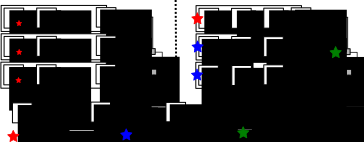
\includegraphics[width=0.45\textwidth]{fig/overview.pdf}
%%
    \caption{ System overview, Metadata, client, and Remote Memory
    servers are Clover components. Our remote memory coordinator is
    located on a centralized TOR interconnecting the clover components.
    }
%%
    \label{fig:overview} 
\end{figure}

\begin{figure}
    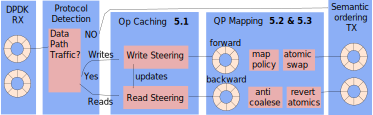
\includegraphics[width=0.45\textwidth]{fig/packet_processing.pdf}
    \caption{Our packet processing pipeline}
    \label{fig:system}
\end{figure}


\subsection{Operation Caching}
\label{sec:operation-caching}

Any asynchronous data structure which allows for lockless reads and writes must
have a mechanism in place to resolve conflicts. When memory is close, conflict
resolution strategies can make many reads and writes quickly in the uncommon
case of a conflict, the cost of which is typically amortized by the unlikelihood
of the conflict itself. In the case of far memory the cost of a conflict is
severe. In contrast to opportunistic algorithms in a shared cache architecture,
in a disaggregated system with small amounts of in network compute conflicts can
be detected and resolved in the data path. Our solution is to provide a general
framework in which developers with knowledge of their remote structures can
resolve their conflicts in network as the operations flow by serially to memory. 

\begin{figure}
    \includegraphics[width=0.45\textwidth]{fig/throughput.pdf}
    \caption{Default Clover throughput vs. Clover with write conflict
    detection and correction turned on \todo{recompute with the read caching values (old)}}
    \label{fig:throughput}
    \vskip -1em
\end{figure}

\subsection{Implementing Atomic replacement}

In the
following subsections we describe the dangers of removing atomics, and present
our solutions.

A few assumptions must be made in order for this replacement of operations to be
made. First and foremost all operation serialization must be made, and finalized
at the point where the CAS is swapped out. More formally, all of the data
structure invariants which required locking, must be satisfied at the time of
transforming the packet. Further the order of operations must be maintained
downstream from the checking of the invariant. These two requirements influence
the design of any system which aims to make this performance improvement.

\textbf{writes:} In the case of clover we cache the location of the latest writes to occur for
each key. If a write occurs which is for a stale virtual address, our conflict
detection algorithm first uses information about clovers algorithm to find the
value of the key in each RDMA write packet. We find this value by checking the
size of the write, and checking the location in the packet for specific clover
data. Once the key from the write is extracted a table lookup is used to
translate the key into the virtual address of the latest write for that key.
This strategy uses 64 bytes per key, as each RDMA virtual address is 64 bytes.
By performing this lookup in the data path all writes succeed regardless of how
contested the memory address is. \todo{ref fig from words}.

\textbf{reads:} Reads present a slightly more complicated case. Writes contain
the key, which allows for a table lookup, while RDMA read requests only contain
a virtual address and a size. When a read fails it must be retried, as mentioned
earlier reads are performed iteratively until the tail of the list is reached,
which in the case of highly contested keys could be arbitrarily long. Repeating
reads does not destroy system performance as they are lockless, however in terms
of client latency each retry adds serious latency. What makes handling reads
hard is identifying the clover key for which the read is for, without additional
data in the packet the value must be determined another way. As reads can be for
arbitrarily old virtual addresses a naieve solution would be to store the entire
lineage of each key, which would require caching all of clovers meta data in the
network. Our solution is to hash the address of each write into an array
~\todo{2x} the size of the keyspace. When writes occur their virtual address and
key value are stored in the array. New writes simply overwrite old values in the
table. This allows keys with higher hit rates to maintain longer histories in
the table. When reads occur their address is looked up in the table, if the
address has a hit the read is steered to the tail of the list. If a miss occurs
the read is left to flow through, clovers default mechanism kicks in and
performs a lookup to the meta data server for the last known address and the
process repeats. We found that by using an array size of 8x the ~\todo{vast
majority of reads succeed first try.} While the number of reads that require a
second try is ~\todo{a number}. ~\todo{insert the CDF of read retries}.

%% ACS - This is just lifted from WORDS; no need to repeat here

%% \begin{figure}
%%     \includegraphics[width=0.45\textwidth]{fig/cache.pdf}
%%     \caption{Performance as a function of keys cached. Caching a few
%%     of the top-$N$ keys provides the greatest marginal throughput
%%     benefits.}
%%     \label{fig:cache}
%% \end{figure}

%% \textbf{reduced cache size} we show that if hot keys are known we require only a
%% small amount of in network state~\ref{fig:cache} we have considered dynamic
%% approaches such as LRU which would allows for a finite amount of space and an
%% arbitrary number of keys to be serviced.

 

\textbf{1) metadata required} The first requirement, that the structural invariants
of the data structure be maintained at the point of transformation demands that
all of the state required to check the structural invariant be present at the
point in the network at which the swap is made. This fact increases the memory
cost on a switch, however with intelligent data structure design the cost of the
required metadata can be mitigated. In the case of Clover, while each key has
an entire linked list history that can potentially span megabytes, the only
required metadata to make the change from CAS to write is the location of the
tail pointer. In this case the metadata cost is O(n) as it grows linearly with
the keyspace.

\textbf{2) reordering} The second requirement, that operations not be reordered
after the invariant has been checked requires more care in real systems. For
instance in an RDMA system with two clients, both could have contesting CAS
operations swapped with writes. As the two clients are transmitting operations on
separate QP, and the receiving NIC makes no guarantees about ordering between QP,
the operations could easily be reordered. In the case with CAS, the order could
be forced by ensuring that if one write was to succeed the second would fail.
Without this guarantee the preservation of operation ordering must be maintained
in another way.

\subsection{Connection Remapping}


Our solution here is simple, given that we have the key's for reads and writes
(Section ~\ref{sec:operation-caching}), all operations for the same key are
mapped to the same QP.  This algorithm requires that a few pieces of state be
maintained per connection.  First the sending and response QP for each sender
and receiver need to be tracked. Second the sequence number of each connection,
and the original message sequence number offset must be maintained. Per client
connection the pair of QP's require 48 bits, and the sequence + message sequence
require an additional 48 for a total of 12 bytes per connection. The storage
requirement for mapped requests varies based on the algorithm. If clients are
able to issue an unbounded number of async requests, then a buffer large enough
to maintain backwards mappings for each request is required. In clover clients
can issue up to 2 async requests, so we keep a two 6 byte mappings for each
connection available to map back. 

Depending on the algorithm and the QP mapping scheme requests from a single
sender can be reordered. That is, if a client makes a read and write request to
different locations in memory, and they are mapped to different QP, they may be
returned out of order. Infiniband allows for out of order operations on
receivers~\cite{infiniband-spec}, which pushes operation ordering to client
side user space. Roce does not allow for out of order operations. In this case
the receiving NIC will retransmit if requests are delivered out of order. Here
we buffer requests in network, as we have application knowledge the size of the
buffer is bounded (to the size of a single read packet in clovers case). We
suggest that given the tight memory restrictions on middleboxes algorithms which
have an unbounded number of async requests leave the ordering of remapped
requests to client side user space using IB verbs or a different transport layer
entirely.

\todo{these sections may not be nessisary}

\subsection{Traffic Identification} Depending on the design of a disaggregated
rack memory traffic might be coresident with regular network traffic.
Additionally some of the traffic on the memory bus may not require tracking or
manipulation. In the case of clover we do not modify any traffic to the metadata
server as it is not in the read/write path. The first stage of our packet
processing pipeline is to match requests for manipulation. In our design users
submit a filter as part of their program to allow traffic which does not need to
be modified to flow freely.

\subsection{Dynamic enable/disable of connections, and epochs} A key goal in our
design is to not require the existence of a middle box in the data structures
algorithm. Clover for instance is designed to deal with memory operations made
to the wrong location via iterative pointer chasing. We strongly suggest that
disaggregated algorithms take this approach as our middlebox solution only acts
to acclerate operations in the common case. We add and subtract connections
based on the send and receipt of a single CAS operation. The QP and sequence
number for the CAS are stored on send, and the ATOMIC ACK is used to retreive
the other recevers QP. As this approach requires only a single packet requests
can be added and removed from our algorithm dynamically with little effort. As
some state may be dependent on the number of connections (such as the key to QP
mappings), state transitions either require a lock, or the coping of current
state over to a new epoch when new connections are added. In all of our
experiments only one such transition is made. We begin our mapping after a
specific number of clients for the experiment have connected. Once the total
number of clients have connected, a switch is flipped, and the QP multiplexing
algorithm begins. Requests which do not have mappings stored, but were in flight
during the flip have their sequence numbers, and MSN values applied to the
connection state of the new epoch.


\section{Implementation}

Our prototype is implemented in a software switch using DPDK, but is designed to
have low memory and computational overhead making it ideal for network devices
such as programmable switches.  RDMA packets are not intended to be modified in
flight, and care must be taken not to corrupt them. RDMA invariant CRCs (ICRC)
are calculated at the time of sending and are designed to ensure the integrity
of the payload. When we modify \texttt{c\&s} packets their ICRC must be
recalculated or the packet will be rejected by the receiving NIC. FPGA
implementations of RDMA ICRC have been built in the past~\cite{Mansour_2019};
the required CRC calculation is identical to Ethernet CRC, with some additional
header components and field masking.  Our DPDK solution uses \texttt{zlib}'s
\texttt{crc32} for the calculation.  We believe that this algorithm can also be
implemented efficiently on a programmable switch.

\section{Evaluation}
\label{s:results}

Adding computation to the network increases latency and consumes memory. Our
evaluation demonstrates that by applying our techniques we are able to see
significant performance boosts in terms of overall throughput, and latency for
existing systems. We discuss the memory implications and show that systems
performance can be significantly improved by replacing compare and swap
operations with writes.

\subsection{Testbed}

Our testbed consists of five machines: a Clover memory server, metadata server,
and two Clover clients; the last machine hosts {\sword}. Physically, the
machines are identical: each is equipped with two Intel Xeon E5-2640 CPUs and
256 GB of main memory evenly spread across the NUMA domains. Each server is
equipped with a Mellanox ConnectX-5 100-Gbps NIC installed in a 16x PCIe slot,
all of which are connected to a 100-Gbps Mellanox Onyx Switch. All Clover
servers are configured with default routing settings: clients send directly to
the metadata and data servers. We install OpenFlow rules on the Onyx switch to
redirect the Clover RDMA traffic to \sword; Figure~\ref{fig:overview} shows the
layout of our testbed.

\subsection{YCSB benchmarks}

\begin{figure*}
    \includegraphics[width=1.0\textwidth]{fig/full_system_performance.pdf}

    \caption{{Performance of {\sword} techniques applied to Clover on YCSB
    benchmarks. The percentage of workload writes increases from left to
    right.}}

    \label{fig:full_system_performance}
\end{figure*}

The YCSB benchmark consists of varying read and write workloads which
have been shown to emulate many common datacenter
operations~\cite{ycsb}. We show how \sword's read and write steering
improve the
%a
%breakdown of our techniques, mainly read and write caching, QP mapping, and
%atomic replacement with respect to their effect to system
performance on two
YCSB benchmarks. We choose YCSB-B (95\% read and 5\% write) as our baseline, and
YCSB-A (50\% read and 50\% write) to demonstrate how our algorithm performs
under high contention.  We also show the performance boosts obtained while
running a 100\% write workload which is intended to emulate other programmatic
workloads which are update heavy.

Figure~\ref{fig:full_system_performance} shows the relative
performance gains from each of \sword's techniques. At 5\% reads write
steering provides minimal performance improvement as the vast majority
of writes succeed on their first try. Individual writes, however, can
lead to many stale reads immediately thereafter which leads write steering
to offer a 1.17$\times$ throughput improvement.
%
%Applying QP mapping to the
%read majorly case adds too much computational overhead to give a
%benefit when writes are low, and only a few compare and swap
%operations exist.
%
At 50\% writes, Clover is well outside of it target workload:
at 64 threads, over half of all write operations fail. Here applying write
steering improves performance by over 1.73$\times$ at 64 threads.

Write steering alone is not sufficient at this level of contention,
however.  Because all writes succeed they easily out-pace reads causing
the majority of reads to fail at 64 threads.  (The resulting impact on
tail latency is clearly shown in Figure~\ref{fig:tail_latency}.)
Applying both read and write steering, on the other hand, yields a
2.82$\times$ throughput improvement as nearly all operations
succeed.

%This workload leads to enough common case failures that
%performance overhead of performing QP mapping still yields a
%performance boost.

Write-only workloads are antagonistic for Clover's optimistic
approach.  Write-only and write+read steering yield 3.89$\times$ and
3.63$\times$ throughput improvements respectively; the read steering
logic is pure overhead due to the complete lack of reads in the
workload.



%%\todo{real takeaways}

% \subsection{Memory Utilization}
% Our techniques give a performance boost at the cost of in network memory. We
% took special care to design our algorithms so that they could 1) use only a
% small amount of network memory, 2) be scalable depending on the resources
% available. We show how our performance varies as a function of the available in
% network state.

% As seen in Figure~\ref{fig:cache} our write caching is able to provide a
% significant performance boost while only using a small number of cached
% addresses. In the following experiment we show the maximum performance boost we
% can provide as a function of the available in network memory. Specifically in
% the case of read and write caching this means shrinking the size of the
% available cache. In terms of QP mapping it restricts the number of connections
% which can have their connections mapped. Unmapped connections must use atomic
% operations for their requests to succeed.

% \begin{figure}
%     \includegraphics[width=0.45\textwidth]{fig/memory_util.jpg}
%     \caption{{Relative performance improvement of our techniques with restricted amounts of memory. Here a rightsized allocation implies that for the given number of connections we could support, all requests were mapped and reads and writes were cached.}}
%     \label{fig:memory_util}
% \end{figure}
%%\todo{say something real about the the memory utilization takeaways}


\subsection{Bandwidth reduction}

\begin{figure}
    \includegraphics[width=0.5\textwidth]{fig/bandwidth_reduction.pdf}
    \caption{Bytes required per operation for each of the three techniques for different write intensities.}
    \label{fig:bandwidth_reduction}
\end{figure}

Placing memory operations in-band with regular network traffic can be
problematic as applications' remote memory usage has the potential to
vary dramatically per application.  Under contention, memory operation
can require additional packet exchanges which inflate the bandwidth
necessary to service the same number of memory requests. Our
in-network steering algorithms remove the need for operations to
retry.

%Figure~\ref{fig:bandwidth_reduction} shows the average bytes
%per Clover operation under three different workloads for default
%Clover as well as {\sword}'s two steering techniques.

We calculate the optimal expected cost of a Clover operation by
averaging the cost of a successful operation across reads and
writes. We get the weighted average by multiplying the cost of a read
and write by the appropriate workload percentage. Each write consists
of an RDMA write followed by a CAS, along with the responses for each
message. A read consists of an RDMA read and read response, and
usually an additional metadata read made asynchronously with the main
read to fetch the latest position of the tail in case the first memory
read fails. Clover performs this second read opportunistically (in
around 99 percent of all reads in these workloads), however sometimes
it is omitted leading to a small over-approximation in our estimate of
``optimal''.

Figure~\ref{fig:bandwidth_reduction} show the average bytes per
operation for each strategy across all three write workloads. We
calculate the value for each technique by summing the total bandwidth
across a run and dividing by the total number of operations. Clover's
bandwidth usage increases with contention, growing by 1.8$\times$ at
50\% and 2.24$\times$ at 100\% writes---all of which is recovered by
applying read and write steering. Write steering alone causes
significant inflation in the cost of operations at 50\% writes because many
read operations fail as discussed above.

\subsection{Tail latency}

\begin{figure*}
    \includegraphics[width=1.0\textwidth]{fig/99th_latency.pdf}

    \caption{Left: Read tail latencies 99th percentile. Right: Write latencies.
    Each measure taken on a Zipf distribution of requests with 64 clients. Note that the y axis is log scale}

    \label{fig:tail_latency}
\end{figure*}

Perhaps the most critical variable that governs overall system
performance is tail latency. In the context of disaggregated memory
systems, reads and writes are often deeply integrated into the
computational logic of a program and the whole program must wait for a
page fault to complete before continuing. We therefore consider poor
tail latency to be a fundamental barrier to the widespread adoption of
far memory systems.  Optimistic concurrency is well known to exhibit
poor tail latency under contention, and Clover is no exception to this
rule. Our techniques significantly reduce tail latency as steering
ensures that nearly all operations succeed with no need to retry.

Figure~\ref{fig:tail_latency} shows the 99th-percentile tail latencies
associated with each of \sword's techniques in comparison with default
Clover. Clover's read latency (left-hand plot) at 5\% reads is
91~$\mu$s, around 7.5$\times$ its baseline our our testbed. With read
and write steering the tail latency of reads drops to 38~$\mu$s---a
2.3$\times$ improvement over Clover even in this low-contention
regime. At 50\% writes the performance increase is roughly double.  As
discussed above, in either case applying write steering alone actually
hurts performance, as it makes reads more likely to fail.
%read performance is improves by 2$\times$
%relative to Clover with the exception of write steering alone. When
%write steering is applied without the aid of read steering the writes
%quickly out-pace the reads, leading the vast majority of reads to fail
%on their first attempt.
Given that these tests were conducted with a
Zipf distribution across 64 cores it is highly likely that more than
one thread is writing to the hottest keys at any point during the
run. This leads some read operations to fail 10s of times before
succeeding.

%Because of this property we suggest
%that read and write steering be used in concert unless the workload is
%explicitly known.

Writes (right-hand side of Figure~\ref{fig:tail_latency}) perform
worse than reads under contention in default Clover. Write+read
steering provides a 2.7$\times$, 37.1$\times$, and 25.2$\times$
improvement in tail latency, respectively, across 5, 50, and 100\%
write workloads.  As one might expect, performing write steering alone
privledges writes over reads, dropping their tail latencies even
further---but likely insufficiently enough to make up for the dramatic
spike in read tail latency

Figure~\ref{fig:tail_latency} also shows the performance of queue pair
mapping and atomic replacement (CAS$\rightarrow$Write) when applied in addition
to write+read steering.  Because the operations are already likely to
succeed, there is no reason to expect any significant drop in tail
latency by vectoring the operations to a particular QP or removing the
CAS guard.  Rather, these plots show that the (significant) additional
logic required in {\sword} to implement these functions result in only
marginal increase in tail latency relative to steering alone---and still
significantly outperforms default Clover.

%The application of QP mapping and swapping
%CNS to writes does little to effect tail latency as their performance
%cost comes largely as an increase to the average.


\subsection{Atomic replacement}

\begin{figure}
    \includegraphics[width=0.5\textwidth]{fig/cas_vs_swap.pdf}
    \caption{Throughput of conflicting CAS and rewritten CAS operations as a function of client threads/QPs.}
    \label{fig:cas_vs_swap}
\end{figure}

We show the ability of swapping compare and swap operations to writes
to overcome hardware atomic bottlenecks by running a micro-benchmark
that focuses exclusively on CAS performance.  Specifically, we extract
the CAS request alone from Clover's write operation (recall it
consists of both an RDMA write and CAS) and repeatedly generate it
from one client to a single memory server (while routing it through
{\sword} as before).

%Here we remove clover from the
%mix and run a simple benchmark of RDMA CAS operations between two
%servers. \sword is routed to via a different set of OpenFlow rules.

Each client thread is bound to a its own queue pair, and all client
threads issue CAS operations to the same shared virtual address.  We
set the number of cores on the {\sword} middlebox to 24 so that in our maximal
test case each client thread flows through exactly one middlebox core
for the lowest degree of interference between QP.

%All requests are routed
%through our middlebox.
In the default case (labeled CAS in Figure~\ref{fig:cas_vs_swap}),
{\sword} lets CAS operations flow through without interference, each
on their own queue pair.  In the CAS$\rightarrow$Write configuration
{\sword} needs to rely upon the ordering semantics of RCs (because all
the operations are for the same memory address and therefore
conflict), so maps all client requests to the same QP at the server.
Due to DPDK queue-to-core partitioning requirements all TX for a
destination QP must be done by a specific core on the
middlebox. Because of this requirement all requests in this
configuration must flow through a single core prior to being issued to
the memory-side NIC.

%all client cores request the same address, and as such all are routed
%onto the same destination QP. Note that this configuration has the
%highest degree of contention for our middlebox as 24 client threads
%must be multiplexed to and from a single client connection. Further

We measure the server throughput in terms of operations per second as
we increase contention by adding client threads.
Figure~\ref{fig:cas_vs_swap} shows the performance gained by
converting CAS operations to writes. Both configurations hit distinct
bottlenecks: CAS operations bottleneck due to being applied to a
single key (c.f. Figure~\ref{fig:rdma_concur}). In the case of
converting CAS to write, the bottleneck is the processing power of the
CPU cores in our DPDK-based {\sword} prototype. (The maximum throughput
our prototype can process is 2.8 million operations per second per
core.)
%In this configuration all
%requests to the memory server must be processed by the same TX
%core. As such our bottleneck is approximately 2.8 MOPS. Hardware
%implemented CRC, cache tuning, and better lock management for TX
%queues could yield higher per core performance in the future.
Despite this implementation restriction, these results clearly show that
replacing CAS with write avoids the memory server NIC's hardware
bottleneck, enabling increased scalability with a more performant
{\sword}---such as one implemented on a programmable switch.

\section{Limitations}

As starkly demonstrated above, the performance  of
our {\sword} prototypes are hardware limited.
%ed as user-space software and not on
%programmable networking hardware.
%There are additional limitations, in terms of language restrictions
%and processing power, which would arise in a full-featured hardware
%implementation. For example, in programmable switches the need to
%recirculate packets which exceed the computational capacity of a
%pipeline results in decreased overall bandwidth.  Prior work on
%programable switches informed our DPDK prototype and led us to 
%avoid design  which would not be implementable on a programmable
%switch.
%

In addition to the challenge of ACK coalescing, a robust connection
multiplexing implementation must support worst-case incast
scenarios where all client requests map to the same connection.
%\textbf{Connection mapping.} Each memory bound RDMA packet
%generates a map entry to demultiplex responses back to its
%original connection. On incast (all clients sending to the
%same resource) a connection must have enough preallocated
%mapped entries in its ring buffer for every connected
%client. 
%%
Because RMT switch registers are allocated at compile time,
statically provisioning for the worst case requires $O(n^2)$
space complexity ($n$ entries for every connection).
%Supporting 512 clients requires 2MB of SRAM (1/16th of
%a Tofino's total buffer space) given this constraint.
%Storing these 64-bit entries takes 2 pipeline stages in the
%best case, and 8 in the worst (8-bit registers).
%In the worst number of in flight requests with $n$ close
%looped clients is $n$, so $n^2$ is dramatic over
%provisioning. However, s
While space-efficient alternatives like hash tables exist,
%tables have much better space utilization, but
collisions
are hard to deal with. For each potential collision,
additional pipeline stages must be allocated and entries
must include QP IDs to check for collisions---increasing a
single hash table lookup to four stages.
%, which is multiplied for each potential collision.
At millions of packets per second multiple collisions are common,
exceeding the pipeline length of our Tofino switches.


Even our P4-based Clover experiments fall short of the underlying NIC hardware
limits.  While our results show significant performance boosts from
reducing hardware contention, there may be additional bottlenecks we
have not yet uncovered. In future work we would like to push the limits of the underlying hardware.
Based on our measurements so far, we expect that higher request rates
will see further benefits from reduced contention.

%~\ref{fig:full_system_performance}.

More generally, some practical aspects of RDMA
interposition---especially under failure and overload---are left out
of this work. For instance, correctly handling ECN packets is a
difficult question when connections are being multiplexed as the
generated ECN packet has a single destination. One option is to
broadcast the ECN to all clients multiplexed on the destination
connection and allow end-to-end congestion control. Another is to track individual client request rates and only issue ECN to the
highest requesting clients. We leave congestion
control implications to future work.

\section{Conclusion}

We leverage the top-of-rack switch to resolve in-network
contention and enable efficient sharing of remote memory.
%for passive remote memory and show that by resolving
%conflicts in flight,
{\sword} can improve the performance of systems that rely on
atomic operations and optimistic concurrency. Our
full-featured prototype demonstrates the potential of
removing atomic operations and relying entirely upon
queue-pair ordering guarantees.  While connection
multiplexing is currently gated by the single-core
performance of DPDK, our P4 steering implementation shows
order-of-magnitude gains in the context of one of the
highest-performing systems available.

% Moreover, we describe how it is
% possible to replace atomic memory operations with traditional reads
% and writes to avoid performance limitations inherent in such
% heavyweight operations.

% \section{Discussion and future work}

Our approach only measures the benefits which clover observers by using our in
network contention resolution. However our approach is general, and in the
future we would like to add functionality for different systems. For example
Remote Regions~\cite{reigons} implements a POSIX file system API for remote
memory.  Our approach could also be used to remove contention here in a much
more standardized remote memory environment.

Clover represents a state of the art key value store for remote memory, however
it is designed with a different set of assumptions than we anticipate for future
systems. We believe that in the context of remote memory with programmable middle
boxes we should architect remote algorithms differently. Mainly that algorithms
and data structures should be designed with the assumption that conflicts can be
resolved using small amounts of high speed compute in network. We aim to explore
the design space of such algorithms and data structures in the future.
%\section*{Acknowledgments}

%\newpage

\balance
\vspace{-0.3cm}
{\footnotesize \bibliographystyle{acm}
%%\bibliography{paper,sysnet}}
\bibliography{paper}}
\vspace{-0.5cm}

\appendix
\section{Appendix}

Here we provide additional evaluation results and details regarding
our implementations.

\subsection{Packet size}

{\sword} is designed to run at line rate, and is unperturbed by packet
size. In the case of Clover, its retries incur a significant bandwidth
overhead which causes additional slowdown when payloads are large.
Figure~\ref{fig:packet_size} shows how {\sword} reacts to changes in
packet sizes. At 128 bytes the limitation is the load applied by
clients. At 256 bytes and above the 100-Gbps limit of the ConnectX-5
NICs becomes the bottleneck for read and write steering, and the
throughput drops proportionally.  Clover retries on larger packets are
more expensive than on smaller packets because the retry consumes
additional bandwidth on an already saturated link.

\begin{figure}
  \centering
  \includegraphics[width=0.485\textwidth]{fig/packet_size.pdf}
\vskip 0.5em
    \caption{Performance across RDMA payload sizes using 400 client cores at a
    50:50 read/write ratio.}
\vskip 0.5em
    \label{fig:packet_size}
\end{figure}

\subsection{Contention}
\label{ss:zipf}

{\sword} is designed to operate well under even extreme contention. We
generate workloads at different points across a Zipf distribution.
The community standard for Zipf is 0.99; at this ratio the most
frequently requested key is requested around 17\% of the time. We
measure further down the distribution up to Zipf of 1.5, at which
point the hottest key is requested over 50\% of the time, and the
second hottest is around 20\%.  Figure~\ref{fig:contention} shows that
in the face of high contention 1.0 and above write and read steering
yields a 40$\times$ and above performance improvement at a 50\% write
workload. The decrease in read and write performance at high
contention is due to Clover's block allocator which becomes a
bottleneck with very hot keys.
%when keys are requests more than 30\% of the time.

\begin{figure}
  \centering
  \includegraphics[width=0.485\textwidth]{fig/contention.pdf}
\vskip 0.5em
    \caption{Performance as a function of Zipf coefficient using 400
    client cores on a 50\% write workload.}
\vskip 0.5em
    \label{fig:contention}
\end{figure}




\subsection{RDMA ICRC}
\label{sec:appendix_icrc}

RDMA requests are not intended to be modified in flight, and care must
be taken not to corrupt them. RDMA invariant CRCs (ICRC) are
calculated at the time of sending and are designed to ensure the
integrity of the payload. When we modify requests their ICRC must be
recalculated or the packet will be rejected by the receiving NIC. Such
an error would cause an extreme performance hit as any dropped packet
triggers a timeout, and go-back-$n$ retransmission.  FPGA
implementations of RDMA ICRC have been built in the
past~\cite{Mansour_2019}; the required CRC calculation is identical to
Ethernet CRC, with some additional \texttt{crc32} for the
calculation. This algorithm is highly optimized for general case CRC
calcuation.

Recalculating the CRC for modified requests is the primary overhead of
{\sword} as it must be recalculated after a squence number update,
which occurs on all multiplexed and demultiplexed requests. This
overhead could be reduced by either removing the need for the CRC
(which is not a feature available on CX series NICs) or by allowing an
alterative, lightweight checksum which could be quickly updated based
on changes made to the packet while in flight. While these options are
not currently available we believe that commodity switches and
SmartNICs could leverage hardware offloads to reduce the cost, as the
CRC calculation is identical to Ethernet except masking
RoCE-specified packet felids.

%% We implemented RDMA ICRC in our DPDK prototype. To our knowledge no P4 switches
%% have native RoCEv2 support, while some projects have demonstrated that it is
%% possible to implement by hand, it requires many switch resources and adds
%% complexity~\cite{p4-telem} we forgot the additional complexity and turned off
%% ICRC checking on our CX5 NICs similar to prior work~\cite{switchml}. In the
%% future we hope that RoCEv2 checksums, like TCP, UDP,and Ethernet checksums can
%% be made hardware primitives on programmable switches.

%% \subsection{CXL} 
%% \label{sec:cxl}

%% CXL is a CPU-to-Device interconnect layered on PCIe 5.0 designed to
%% provide a coherent interface to devices, accelerators and
%% memory~\cite{cxl-spec}.  Although at the time of writing CXL is not a
%% commercially available technology, research prototypes have have
%% reported remote memory access latencies between
%% 200-426ns~\cite{direct-cxl,microsoft-cxl-first-gen,facebook-cxl-tpp}.

%% CXL removes the DIMM slot constraint on per server memory capacity and provides
%% a way forward for high capacity memory pooling between many CPUs. The CXL
%% protocols do not provide opportunities for reducing or removing contention to
%% shared memory.  CLX.cache for instance exposes MESI states to the host CPU, and
%% levees coordination to them. This interface suggests that CXL devices will
%% suffer from identical lock contention problems as traditional memory with
%% inflated costs for coordination. Given that PCIe root complexes lack
%% programmability our techniques will likely not be applicable to CXL. We leave
%% resolving CXL memory contention to future work.


\end{document}
